% --------------------------------------------------------------------
% This is a simple Beamer document that uses beamerthemesigma.sty
% Reading the comments should help you create a presentation even if
% you've never used Beamer before.
% --------------------------------------------------------------------
% Set our document class to Beamer

% add [handout] to class options to turn off \pause behavior 
% this is ideal for slides posted on website/on #slides in 
% the Discord
\documentclass[aspectratio=169, handout]{beamer}

% Some packages for nice font encodings in the final PDF
\usepackage[utf8]{inputenc}
\usepackage[T1]{fontenc}

% To insert images
\usepackage{graphicx}

% Useful packages from the AMS
\usepackage{amsmath,amssymb,amsthm}

% From Jeff E
\usepackage{algo}

% Package for code highlighting
\usepackage{minted}
\setminted{linenos=true, breaklines=true, breakanywhere=true, style=default}
\usemintedstyle{monokai}

% Pretty tables
\usepackage{booktabs}

% Set a title
\title{Welcome To SIGma}

% The subtitle is generally where I'd expect you to put the week
% number, thus:
\subtitle{Week 0}

% Whoever worked on the presentation:
\author{SIGma}

% A date, if you'd like.
\date{}

% An institute name, if you're so inclined
% \institute{University of Illinois Urbana-Champaign}

% Use the SIGma theme for this Beamer presentation
\usetheme{sigma}
% --------------------------------------------------------------------
% Begin document
\begin{document}

% Beamer calls each slide a "frame", defined within the environment:
% \begin{frame}
%   <frame content here>
% \end{frame}

% This frame is just the title.
\begin{frame}
\titlepage
\end{frame}

% A frame with the table of contents.
% This frame's title is "Outline".
\begin{frame}{Outline of a Short Meeting}
  \tableofcontents
\end{frame}


\section{Officers in No Particular Order}

% Officer type people put info here
\begin{frame}{Anakin (\texttt{@Spamakin})} 
        \begin{itemize}
        \item Math Major
        \item SIGPwny Crypto\footnotemark\ Gang + Admin team
        \item CA for CS 173 + 374
        \item Research with Sam
        \item Intern at CME Group over the summer
    \end{itemize}
    \footnotetext[1]{Not that one, the other one}
\end{frame}

\begin{frame}{Sam (\texttt{@Surg})}
    \begin{itemize}
        \item Summer Amazon Intern
        \item CS Major
        \item Doing CS374 Course Dev
        \item Doing Theory Research with Sariel Har-Peled
        \item Research with Anakin
    \end{itemize}
\end{frame}

\begin{frame}{Husnain}
\begin{itemize}
    \item Math Major
    \item SIGPwny Crypto Gang + Helper
    \item Project Euler Enthusiast
\end{itemize}
\end{frame}

% I'll introduce Husnain and Sam since they won't be here

\begin{frame}{Aditya (\texttt{@nebu})}
    \begin{itemize}
        \item ECE/Math double degree.
        \item Worked on fast Ethernet error correction hardware over the summer.
        \item Other interests: FP, PL, Crypto.
    \end{itemize} 
\end{frame}

\begin{frame}{Hassam}
    \begin{itemize}
        \item Intern at Amazon over the summer
        \item CS/Math Dual Major
        \item SIGPwny Crypto Gang + Admin team
        \item CA for CS 233
        \item Compiler research
    \end{itemize}
\end{frame}

\begin{frame}{Phil (\texttt{@fizzle})}
    \begin{itemize}
        \item CS/Ling Major
        \item CA for CS 233
        \item SIGecom - game theory, economics, and computation
    \end{itemize}
\end{frame}

\section{Computing Fibonacci}
\frame{\sectionpage}

\begin{frame}{Recursive}
    
    $$
        F_{n+1} = F_n + F_{n - 1}\quad (n \geq 1; F_0 = 0; F_1 = 1)
    $$
    
\end{frame}

\begin{frame}{}
    \begin{figure}
        \centering
        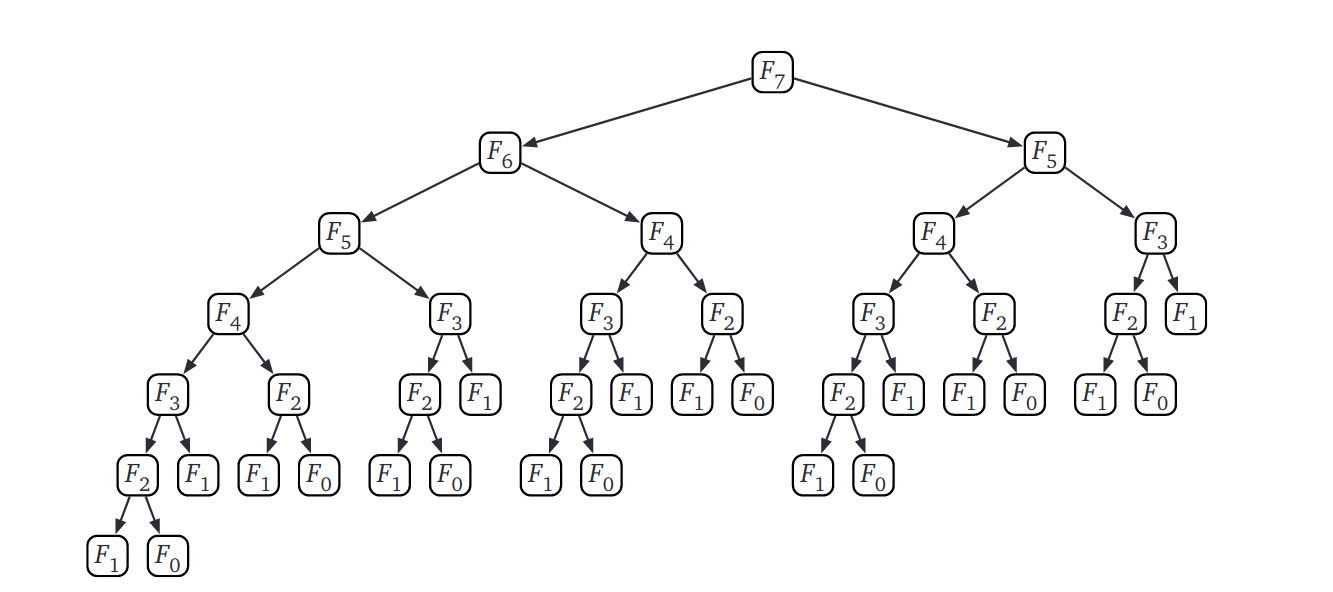
\includegraphics[scale=0.4]{F7_Recursion.png}
        \caption{From Algorithms by Jeff Erickson}
    \end{figure}
\end{frame}

\begin{frame}{Iterative}
    \begin{algo}
        \textul{\textsc{fibonacci}(n):}\+
    \\      $prev, curr \gets 1, 0$ 
    \\      for $i \gets 1 \ldots n$\+
    \\          $next \gets curr + prev$
    \\          $prev \gets curr$
    \\          $curr \gets next$\-
    \\      return $curr$
    \end{algo}
\end{frame}

\begin{frame}{Aside: Square-and-Multiply}
    Before we get to the even faster way to compute $F_n$, we first look how to compute powers of a number quickly.
    
    Say we want to compute $x^8$. We can use 7 multiplications as follows: 
    $$x \to x^2 \to x^3 \to x^4 \to x^5 \to x^6 \to x^7 \to x^8$$ 
    
    \pause
    
    But we can use just 3: 
    $$x \to x^2 \to x^4 \to x^8$$.
    
\end{frame}

\begin{frame}{}
    We can use 12 multiplications to compute $x^{13}$ as follows: 
    $$x \to x^2 \to x^3 \to x^4 \to x^5 \to x^6 \to x^7 \to x^8 \to x^9 \to x^{10} \to x^{11} \to x^{12} \to x^{13}$$ 
    
    \pause
    
    But if we first compute powers as such
    \begin{align*}
        x^2 &\gets x \cdot x \\
        x^4 &\gets x^2 \cdot x^2 \\ 
        x^8 &\gets x^4 \cdot x^4 \\
    \end{align*}
    
    \pause
    
    And then using these we get $x^8 \cdot x^4 \cdot x = x^{13}$ in just 6 total multiplications.
    
    \pause
    
    We can generalize this using binary    
    \begin{table}[]
    \begin{tabular}{|l|l|l|l|}
    \hline
    \textbf{1} & \textbf{1} & 0 & \textbf{1} \\ 
    \hline
    \end{tabular}
    \end{table}
\end{frame}


\begin{frame}{}
\begin{figure}[htbp]
 \begin{minipage}{0.5\linewidth}
  \centering
    \begin{algo}
        \textul{\textsc{power}(\emph{x, n})}:\+
    \\  $curr \gets 1$
    \\  for $i \gets 1 \ldots n:$\+
    \\      $curr \gets curr * x$\-
    \\  return $curr$

    \end{algo}
 \end{minipage}%
 \pause % Honestly impressive that this works
 \begin{minipage}{0.5\linewidth}
  \centering
    \begin{algo}
        \textul{\textsc{squareMultPower}(x, n):}\+
    \\      $res, power \gets 1, x$
    \\      for bit in \textsc{binary}(n):\+
    \\          if bit = 1:\+
    \\              $res \gets res * power$\-
    \\          $power \gets power * power$\-
    \\      return $res$
    \end{algo}
 \end{minipage}
\end{figure} 

\end{frame}

\begin{frame}{Matrices}
    We have the following two linear equations
    \begin{align*}
        F_n &= F_{n - 1} + F_{n - 2} \\
        F_{n - 1} &= F_{n - 1} \\
    \end{align*}
    
    \pause
    
    We can represent this as follows using matrices
    % Worlds worst line of tex down here
    $$\begin{bmatrix} F_{n - 1} \\ F_{n} \\ \end{bmatrix} = \begin{bmatrix} 0 & 1 \\ 1 & 1 \\ \end{bmatrix} \begin{bmatrix} F_{n - 2} \\ F_{n - 1} \\ \end{bmatrix} \pause = \begin{bmatrix} 0 & 1 \\ 1 & 1 \\ \end{bmatrix}^2 \begin{bmatrix} F_{n - 3} \\ F_{n - 2} \\ \end{bmatrix} \pause = \ldots = \begin{bmatrix} 0 & 1 \\ 1 & 1 \\ \end{bmatrix}^n \begin{bmatrix} 0 \\ 1 \\ \end{bmatrix}$$
    
\end{frame}

\begin{frame}{Generating Functions}
    \begin{quote}
        ``A generating function is a clothesline on which we hang up a sequence of numbers for display'' 
    \end{quote}
    % There's probably a better way to do this but whatever
    \hfill\textbf{--- Herbert Wilf}, \emph{Generatingfunctionology} 
\end{frame}


\begin{frame}{Generating Functions}
    Explicitly, our recurrence is
    $$F_{n+1} = F_n + F_{n-1}\quad (n \geq 1; F_0 = 0; F_1 = 1)$$
    \pause
    Define a ``generating function'': a function whose coefficients are the Fibonacci numbers
    $$F(x) = \sum_{n\geq 0} F_n x^n = F_0 + F_1x + F_2x^2 + \cdots$$
    Let's find this function!
\end{frame}

\begin{frame}{Generating Functions: The LHS}
Given,
\begin{align*}
    &F(x) = \sum_{n\geq 0} F_n x^n\qquad
    F_{n+1} = F_n + F_{n-1}\quad (n \geq 1)
    \end{align*}\pause
     Multiply LHS of recurrence by $x^n$, and take the sum for $n \geq 1$.
     \begin{equation}
     F_2x + F_3x^2 + F_4x^3 + \cdots = {\color{sigma@mainblue} {\frac{F(x) - x}{x}}}
     \end{equation}
\end{frame}

\begin{frame}{Generating Functions: The RHS}
Given,
\begin{align*}
    &F(x) = \sum_{n\geq 0} F_n x^n\qquad
    F_{n+1} = F_n + F_{n-1}\quad (n \geq 1)
    \end{align*}\pause
     Multiply RHS of recurrence by $x^n$, and take the sum for $n \geq 1$.
     \begin{align*}
     &\left( F_1x + F_2x^2 + F_3x^3 + \cdots \right) + \left( F_0x + F_1x^2 + F_2x^3 + \cdots \right)\\[1em]
     &= {\color{sigma@mainblue} F(x) + xF(x)}{\addtocounter{equation}{1}\tag{\theequation}}
     \end{align*}
\end{frame}

\begin{frame}{Generating Functions: Equate LHS and RHS}
\begin{align*}
    &\frac{F(x) - x}{x} = F(x) + x \cdot F(x)\\[1em]
    \implies & F(x) = \frac{x}{1-x-x^2}
\end{align*}
That's our generating function!
% the nth Fibonacci number, F_n, is the coefficient of x^n in the expansion of the function x/(1 − x − x^2) as a power series about the origin
\end{frame}

\begin{frame}{Generating Functions: Some Further Analysis}
    Remember partial fraction decomposition?
    $$F(x) = \frac{x}{1-x-x^2}$$
    \pause
    
    $$F(x) = \frac{x}{(1-xr_+)(1-xr_-)} = \frac{1}{r_+ - r_-}\left( 
        \frac{1}{1-xr_+} - \frac{1}{1-xr_-}
    \right)$$
    where
    $$r_\pm = \frac{1\pm \sqrt{5}}{2}$$
\end{frame}

\begin{frame}{Generating Functions: Geometric Series}
For a geometric series,
$$\sum_{n=0}^\infty ar^n = \frac{a}{1-r}$$\pause
    Using the geometric series sum formula,
    $$F(x) = \frac{1}{\sqrt{5}}\left( 
        \frac{1}{1-xr_+} - \frac{1}{1-xr_-}
    \right)$$\pause
    $$\implies F(x) = \frac{1}{\sqrt{5}}\left(\sum_{i= 0}^\infty r^i_+x^i -  \sum_{i= 0}^\infty r^i_-x^i\right)$$
\end{frame}

\begin{frame}{Generating Functions: Almost There}
 Writing this out to make it a bit more obvious,
 $$F(x) = \frac{1}{\sqrt{5}} \left(\sum_{i = 0}^\infty (r^i_+ - r^i_-)x^i  \right)$$\pause
 Doesn't this look a lot like a polynomial? 
 The coefficients are the Fibonacci numbers we are after!
\end{frame}

\begin{frame}{Generating Functions: Closed Form}
    Picking off coefficients from the geometric series, we see that
    
    $$F_n = \frac{1}{\sqrt{5}}\left(r_+^n - r_-^n \right)$$\pause
    
    Since $|r_-/\sqrt{5}| < 0.5$ for all $n \geq 0$, we can actually neglect it altogether to get a simpler closed form:
    
    $$\color{sigma@mainblue} F_n = \left\lfloor\frac{1}{\sqrt{5}}\left(\frac{1+\sqrt{5}}{2} \right)^n\right\rceil$$
    
\end{frame}

\begin{frame}{Summary}
\centering
    \begin{tabular}{@{}lr@{}}
    \toprule
        Algorithm & Time Complexity \\
    \midrule
        Naive recursive      & $O\left( 2^n \right)$\\
        Iterative            & $O(n)$\\
        Matrix               & $O(\log n)$\\
        Generating functions & $O(1)$\\
    \bottomrule
    \end{tabular}
    
    
\end{frame}


\section{Open Forum}
\frame{\sectionpage}

\begin{frame}
    \Huge{\centerline{Time?}}
\end{frame}

\begin{frame}
        \Huge{\centerline{Book?}}
\end{frame}

\begin{frame}
        \Huge{\centerline{Research?}}
\end{frame}



% There's a way to automate this, see:
% https://tex.stackexchange.com/questions/178800/creating-sections-each-with-title-pages-in-beamers-slides/178803

\begin{frame}
  \begin{center}
    {\color{sigma@mainblue} So long, and thanks for all the fish!}
  \end{center}
\end{frame}

\end{document}